%!Tex Root = ../main.tex
% ./Packete.tex
% ./Design.tex
% ./Deklarationen.tex
% ./Vorbereitung.tex
% ./Aufgabe1.tex
% ./Aufgabe3.tex
% ./Aufgabe4.tex
% ./Bonus.tex

\section{Aufgabe 2}

\setcounter{task}{1}

\begin{frame}[allowframebreaks]{Task 2}{Isomorphisms}
  \begin{requirementsnoinc}
    \begin{columns}
      \begin{column}{0.5\textwidth}
        \ctikzfig{2a_1}
      \end{column}
      \begin{column}{0.5\textwidth}
        \ctikzfig{2a_2}
      \end{column}
    \end{columns}
  \end{requirementsnoinc}
  \begin{solutionnoinc}
    \begin{columns}
      \begin{column}{0.5\textwidth}
        \ctikzfig{2a_1_sol_2}
        % ./figures/2a_1_sol_2.tikz
      \end{column}
      \begin{column}{0.5\textwidth}
        \ctikzfig{2a_2_sol_2}
        % ./figures/2a_2_sol_2.tikz
      \end{column}
    \end{columns}
    \vspace{0.5cm}
    \begin{enumerate}
      \item look at \alert{degree} of vertices
      \item[]
    \end{enumerate}
  \end{solutionnoinc}
  \begin{solution}
    \begin{columns}
      \begin{column}{0.5\textwidth}
        \ctikzfig{2a_1_sol}
        % ./figures/2a_1_sol.tikz
      \end{column}
      \begin{column}{0.5\textwidth}
        \ctikzfig{2a_2_sol}
        % ./figures/2a_2_sol.tikz
      \end{column}
    \end{columns}
    \vspace{0.5cm}
    \begin{enumerate}
      \item look at \alert{degree} of vertices
      \item search for \alert{subgraphs} / \alert{cycles}
    \end{enumerate}
  \end{solution}
  \begin{requirementsnoinc}
    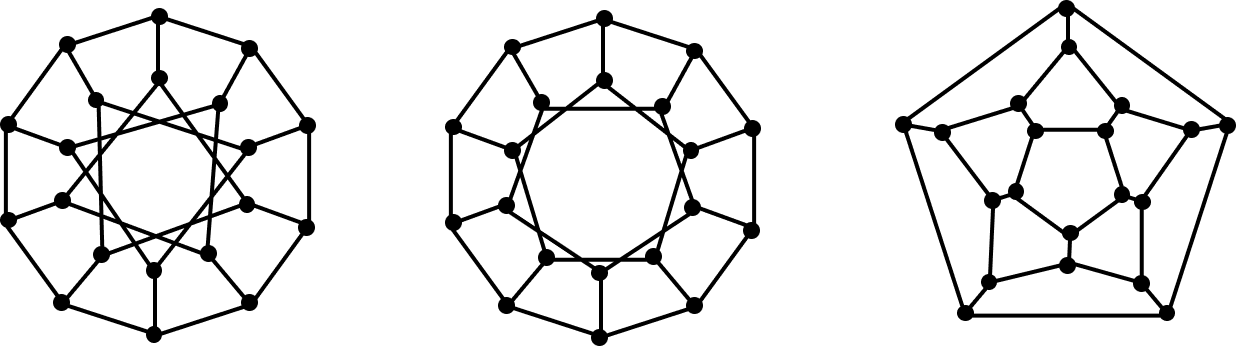
\includegraphics[width=\textwidth]{./figures/isomorphism2.png}
    \begin{itemize}
      \item asdf
    \end{itemize}
  \end{requirementsnoinc}
  \begin{solution}
    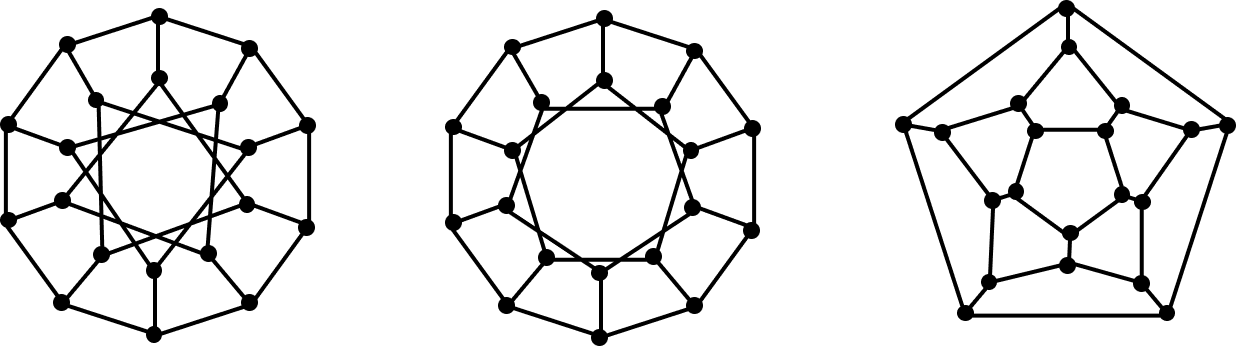
\includegraphics[width=\textwidth]{./figures/isomorphism2.png}
  \end{solution}
\end{frame}
